\begin{flushright} {\tiny {\color{gray} surfaceprocesses.tex}} \end{flushright}

%.......................................................................
\subsubsection{In 1D - simple nonlinear diffusion a la Burov \& Cloetingh \cite{bucl97}}

The tectonic-scale transport equations describe long term changes
in topography $h(x,y,t)$ as a result of simultaneous short- and long-range
mass transport processes \cite{befh92,kobe94}.

The short-range surface processes are represented by cumulative effects of hillslope 
processes (soil creep, rainsplash, slides) that remove material from uplifted areas 
down to the valleys. 
It is then assumed that the horizontal material flux $\vec{q}_s$ is related to 
local slope $\vec\nabla h$ by $\vec{q}_s=-K_s \vec{\nabla}h$ 
where $K_s$ is the effective diffusivity. Assumption of conservation of mass 
volume leads to the linear diffusion equation for erosion:
\[
\frac{\partial h}{\partial t} = K_s \Delta h
\]
This equation can be solved with constant-elevation (fixed $h$ value)
boundary conditions simulating local base levels of erosion. 

Note that is practice the coefficient $K_s$ might depend on slope and curvature, 
i.e.
\[
\frac{\partial h}{\partial t} = K_s(x,y,h,\vec\nabla h)\Delta h
\]
Following \cite{goss76}, Burov \& Cloetingh use an empirical non linear 
expression $K_s=k_s(x) (\vec\nabla h)^n$. 




%...........................................................
\subsubsection{In 1D - not so simple, a la Andr\`es-Martinez et al\cite{anpa19}}. 

The change in surface elevation rate due to surface processes is equal
to the divergence of the sediment flux 
(assuming there is no density difference between the bedrock and
sediment and ignoring the effects of compaction):
\[
\frac{\partial h}{\partial t} = -\frac{\partial q_s}{\partial x}
\]
where $h$ is the topography, $t$ is the time, $q_s$ represents the sediment flux, 
and $x$ is the horizontal coordinate. 

The next step consists in a formulation for the sediment flux. Still following \cite{anpa19}, 
in the subaerial environment, it is possible to define the sediment transport 
flux $q_s$ in terms of the water flux $q_w$ as
\[
q_s=-(K+c q_w^n) \frac{\partial h}{\partial x}
\]
where $K$ is the slope diffusivity, $c$ is the transport coefficient, 
and $n \geq 1$ is the power law that defines the type
of relationship between the sediment transport and the water flux 
(Simpson \& Schlunegger, 2003; Smith \& Bretherton, 1972).
\todo[inline]{get these papers}
This model accounts for hillslope diffusion processes where the topography will tend to
a dispersive diffusion (Culling, 1960) and fluvial transport processes that result in concentrative diffusion
due to water run off (Graf, 1984). For a simple parameterization we choose a linear relationship between
sediment transport and water flux $(n=1)$.

The water flux can be related to the water discharge/effective rainfall $\alpha$ as
\[
\frac{\partial}{\partial x} (\vec{n} q_w) = -\alpha
\]
where $\vec n$ is a unit vector directed down the surface gradient (Smith \& Bretherton, 1972). 
By assuming a constant $\alpha$ and integrating equation (12) over the surface in the downstream direction, we obtain

\[
q_w = \alpha x_d
\]
where $x_d$ is the downstream distance from the drainage divide. By substituting equations (11) and
(13) into (10) we obtain the 1-D sediment mass conservation equation for combined hillslope and
discharge-dependent fluvial transport
\[
\frac{\partial h}{\partial t} = \frac{\partial}{\partial x} \left( (K+k \alpha x_d) 
\frac{\partial h}{\partial x}   \right)
\]
where the downstream distance $x_d$ is calculated at each time step as the distance from the topographic highs
to the valley floors. Because $q_w$ is dependent on the length of the drainage, the model mimics 1-D landscapes
similar to river profiles in which fluvial processes are dominant.

%...........................................................
\subsubsection{Examples in the literature}

\begin{center}
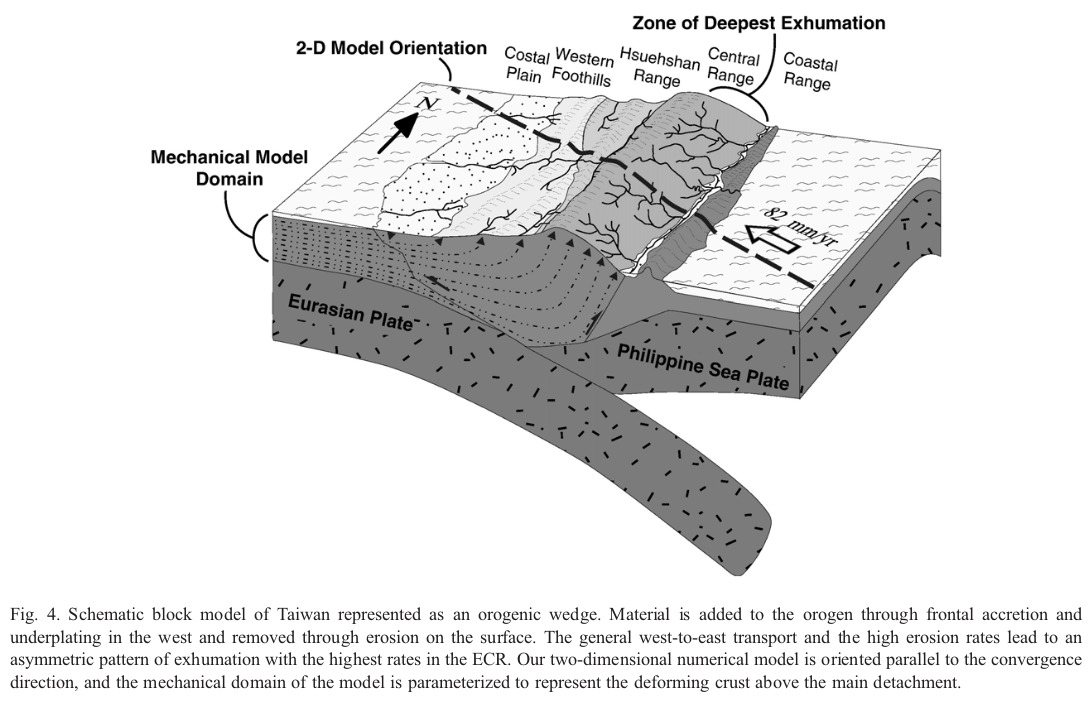
\includegraphics[width=7cm]{images/surfaceprocesses/fuwf06a}
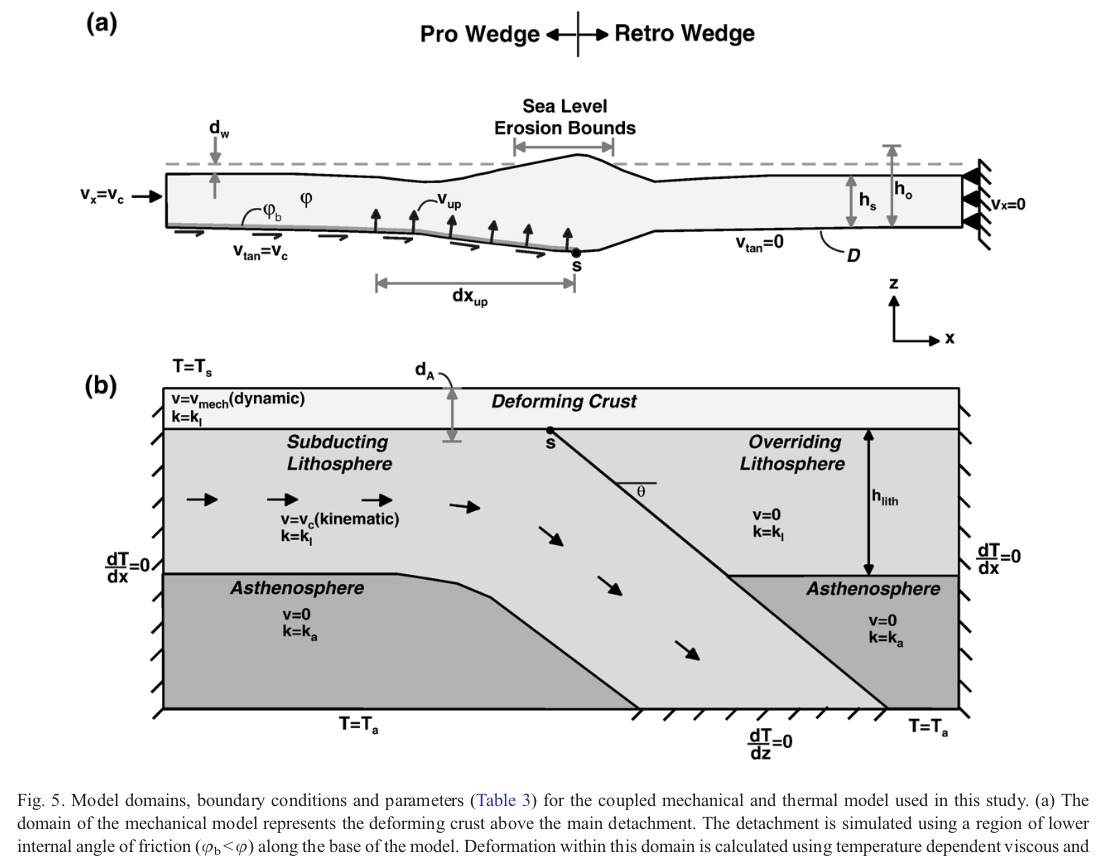
\includegraphics[width=7cm]{images/surfaceprocesses/fuwf06b}\\
{\captionfont Application to Taiwan. Taken from Fuller et al (2006) \cite{fuwf06}}
\end{center}


